\chapter{Introduction \label{chp1}}

Write your introduction chapter here. I have left a few sections from my
dissertation just as an example. Just delete them or modify them as you
see fit.

\section{Motivation}

Here is an example section of a chapter. It includes a figure with caption and
label as well as a citation from the .bib file for this chapter which is named
``intro.bib''. Here is a reference to Figure \ref{exampleFig}.  The caption for
Figure \ref{exampleFig} has an exampel citation.

\begin{figure}[!ht]
    \centerline{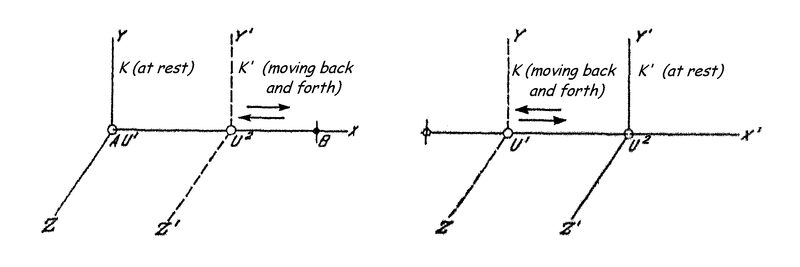
\includegraphics[width=5.0in]{figures/chp1/exampleFig.png}}
    \caption{This figure comes from a paper written by Albert Einstein which I
    will cite here \cite{einstein1916foundation}.  \label{exampleFig}}
\end{figure}

You can create other directories in the ``figures'' directroy for the other
chapters in your disseration if you would like. This just helps keep things
organized.


\section{Dissertation Objectives}

Its a good Idea to list the research objectives. Here is a way you can do it
in a list.
\begin{enumerate}
        \item Description of first objective corresponding to your first paper
            which is included as chapter 4. I can add labels to almost anything
            and reference them at other places in the text. Just make sure all
            your labels are unique throughout all of your included .tex
            documents \label{obj1}
        \item Description of next objective also corresponding to your first
            paper. \label{obj2}
        \item Description of your third objective which might correspond to your
            second paper presented in Chapter 5. \label{obj3}
\end{enumerate}

After this list I can reference objectives \ref{obj1} - \ref{obj3} like this.

\section{Dissertation Structure}

Its also good to include a description of the structure of your dissertation
like what chapters include what info etc. You might do that here.

% this is where the bibliography is included. Just add your bibtex citations
% to the intro.bib file and don't modify the code below unless you want to use
% a different citation style instead of "unsrtnat".
\singlespacing
\bibliographystyle{unsrtnat}
\bibliography{chapters/chapter1/intro}
\doublespacing
